% filepath: /home/oliver/text-learning/documents/math4ml_report/project_report.tex
\documentclass[12pt,a4paper]{article}
\usepackage[utf8]{inputenc}
\usepackage[english]{babel}
\usepackage{amsmath,amsfonts,amssymb}
\usepackage{graphicx}
\usepackage{float}
\usepackage{hyperref}
\usepackage{geometry}
\usepackage{algorithm}
\usepackage{algorithmic}
\usepackage{cite}
\usepackage{subfigure}
\usepackage{booktabs}

\geometry{margin=1in}
\title{Knowledge Discovery in Text Corpora with Diffusion Maps and Information Theory}
\author{Oliver Kirsten}
\date{\today}

\begin{document}

\maketitle

\section{Introduction}

The analysis of document complexity and semantic relationships in large text corpora requires methods that can capture both the hierarchical nature of knowledge and the asymmetric dependencies between concepts. Traditional text mining approaches treat document similarity as a symmetric problem, failing to model the fundamental asymmetries inherent in knowledge representation and learning pathways.

This work introduces a novel framework that combines information-theoretic measures with diffusion geometry to reveal the intrinsic complexity structure of document collections. Our approach leverages cross-entropy kernels to capture asymmetric semantic relationships and SVD-based entropy measures to characterize document complexity along a generality-specialization spectrum.

\subsection{Problem Statement}

The central challenge in knowledge discovery from text corpora lies in understanding how documents relate to each other not just in terms of topical similarity, but in terms of conceptual complexity and prerequisite relationships. Traditional similarity measures face several critical limitations: symmetric distance metrics cannot capture the directional nature of knowledge dependencies (e.g., that advanced concepts require foundational knowledge but not vice versa), existing complexity measures rely on surface-level features like document length rather than semantic depth, standard clustering approaches fail to preserve the hierarchical structure inherent in knowledge domains, and current methods lack principled approaches for discovering learning pathways between conceptually distant topics.

These limitations are particularly pronounced in educational and technical domains where understanding complexity gradients and conceptual dependencies is crucial for effective knowledge organization.

\subsection{Proposed Approach}

Our framework addresses these challenges through three key ideas. First, we introduce SVD entropy as a compression-based measure of document complexity that distinguishes between general foundational content and specialized technical material based on vocabulary distribution patterns in the semantic space. Second, we develop asymmetric cross-entropy kernels that measure the information cost of encoding one document using another's vocabulary distribution, naturally capturing directional semantic relationships and prerequisite dependencies. Third, we combine these information-theoretic measures with diffusion geometry to compute semantic geodesics that represent optimal learning pathways through the knowledge space, respecting both complexity gradients and conceptual relationships.

This approach enables the discovery of natural progression sequences in knowledge domains while providing quantitative characterization of document complexity.

\section{Data}

\subsection{Dataset Description}

The dataset used in this study is derived from the OpenWeb-Math \cite{grosset2021openwebmath} corpus, specifically filtered and curated for mathematical machine learning content. The data collection and preprocessing pipeline involved several stages:

\textbf{Source Selection:} Documents were extracted from the OpenWeb-Math dataset with URL filtering restricted to sources including "wikipedia.org", "github.io", and "nature.com".

\textbf{Topic-based Retrieval:} Zero-shot BERTopic \cite{grootendorst2022bertopic} was employed to retrieve documents matching specific mathematical and machine learning topics, including linear algebra, statistics, probability theory, information theory, machine learning, deep learning, statistical learning, reinforcement learning, and neural networks.

\textbf{Preprocessing Pipeline:} Retrieved documents underwent standard NLP preprocessing techniques including tokenization, stopword removal, and stemming to prepare the text for subsequent analysis.

Each document contains text content, URL, and topic classification, with topics ranging from basic concepts like "Introducing matrices" to advanced topics like "LSTM networks".

\subsection{Data Properties}

This dataset provides an ideal testbed for evaluating semantic relationships and learning pathways in mathematical and machine learning concepts. The hierarchical nature of mathematical knowledge, from foundational linear algebra to advanced neural architectures, allows us to validate whether our diffusion geodesics capture meaningful semantic progressions.

The documents vary significantly in complexity and abstraction level, providing a natural gradient for testing our entropy-based characterization methods. Furthermore, the well-defined conceptual relationships in mathematics and machine learning enable qualitative validation of discovered semantic paths.

\section{Methods}

\subsection{Text Preprocessing and Vectorization}

Our pipeline begins with text preprocessing and Frequency-Inverse Document Frequency (TF-IDF) \cite{salton1988term} vectorization:

\begin{equation}
\mathbf{X}_{t,d} = \text{TF}(t,d) \cdot \log\left(\frac{N}{|\{d' : t \in d'\}|}\right)
\end{equation}

where $t$ represents a term, $d$ a document, and $N$ the total number of documents. The preprocessing includes removal of terms appearing in more than 50\% of documents and terms appearing in fewer than 5 documents, along with Gensim preprocessing for text cleaning.

\subsection{Singular Value Decomposition}

To manage computational complexity while preserving semantic information, we apply SVD:

\begin{equation}
\mathbf{X} = \mathbf{U}\mathbf{\Sigma}\mathbf{V}^T
\end{equation}

where $\mathbf{X} \in \mathbb{R}^{n \times m}$ is the TF-IDF matrix, and we retain the top $k = 5000$ components. This decomposition is also known as Latent Semantic Analysis \cite{deerwester1990indexing}, and provides dimensionality reduction from vocabulary size to manageable dimensions, noise reduction through low-rank approximation, and computational efficiency for subsequent operations.
\subsection{Non-negative SVD (NN-SVD) Transformation}

Since diffusion processes require non-negative values, we apply a Non-negative SVD (NN-SVD) \cite{boutsidis2008svd} transformation that preserves the dominant singular vector components while ensuring non-negativity. This transformation also serves as an effective initialization strategy for Non-negative Matrix Factorization (NMF).

The NN-SVD approach addresses the fundamental challenge that standard SVD produces factors with both positive and negative entries, while many applications (including diffusion processes and NMF) require non-negative representations. For each singular vector component, we preserve the orientation that captures the majority of the signal energy:

\begin{equation}
\mathbf{U}_{\text{nonneg}}[:,i] = \begin{cases}
\max(\mathbf{U}[:,i], \epsilon) & \text{if } \|\mathbf{U}_{+}[:,i]\|_2 \geq \|\mathbf{U}_{-}[:,i]\|_2 \\
\max(-\mathbf{U}[:,i], \epsilon) & \text{otherwise}
\end{cases}
\end{equation}

where $\mathbf{U}_{+}$ and $\mathbf{U}_{-}$ denote positive and negative components respectively, and $\epsilon = 10^{-5}$ prevents numerical issues.

This transformation strategy offers several advantages. Energy preservation is achieved by selecting the orientation with larger $L_2$ norm, retaining the maximum amount of information from each singular vector while satisfying non-negativity constraints. The approach maintains the semantic structure captured by SVD while enabling probabilistic interpretations required for diffusion analysis.

\subsection{Entropy-based Similarity Kernel}
The NN-SVD matrix fundamentally serves as a change of basis for the original TF-IDF matrix, projecting the document representations from the high-dimensional vocabulary space into a lower-dimensional semantic space with non-negative coordinates.

The NN-SVD provides a new basis where each document is represented as:

\begin{equation}
\mathbf{X}_{\text{nonneg}} = \mathbf{U}_{\text{nonneg}}^T \mathbf{X}
\end{equation}

where $\mathbf{U}_{\text{nonneg}}$ forms the new basis vectors derived from the non-negative transformation of the left singular vectors.

We normalize the transformed non-negative matrix to form probability distributions:

\begin{equation}
\mathbf{P} = \frac{\mathbf{X}_{\text{nonneg}}}{\sum_{i} \mathbf{X}_{\text{nonneg}}[i,:]}
\end{equation}

and compute a cross-entropy based kernel:

\begin{equation}
\mathbf{K}_{ij} = -\sum_{k} \mathbf{P}_{ik} \log_2(\mathbf{P}_{jk})
\end{equation}

\subsubsection{SVD Entropy as Document Generality and Complexity Measure}

The SVD entropy provides a novel characterization of document generality through the fundamental principle that \textbf{documents using common, widely-shared vocabulary can be more efficiently compressed using the dominant SVD components, while documents with specialized vocabulary require more components for accurate representation}.

\begin{equation}
H_{\text{SVD}}(d) = \frac{\mathbf{K}_{dd}}{\log_2(n)}
\end{equation}

This measure captures document characteristics along multiple dimensions. Documents with low SVD entropy exhibit high generality, extensively using vocabulary patterns captured by the top SVD components. These documents employ common terminologies and conceptual frameworks found across the corpus, typically representing introductory material, overviews, or foundational concepts that can be efficiently "explained" using the dominant semantic patterns in the corpus. Examples include basic tutorials, general introductions, and widely-applicable principles.

Conversely, documents with high SVD entropy demonstrate high specialization, requiring many SVD components for accurate reconstruction. These documents use terminology and conceptual patterns that are rare or unique within the corpus, representing advanced, specialized, or highly technical content that cannot be efficiently compressed using only the dominant corpus-wide patterns. Examples include research papers, technical specifications, and domain-specific advanced discussions.

The compression-based intuition reveals that SVD entropy directly measures how "compressible" a document is using the corpus-wide semantic patterns. Just as simple images with common features compress well with few JPEG coefficients while complex images with unique details require many coefficients for faithful reproduction, general documents using common vocabulary patterns compress well with few SVD components (low entropy) while specialized documents with unique terminology require many SVD components (high entropy).

This measure has important pedagogical implications, automatically identifying documents by their position in the learning hierarchy. Low entropy documents often represent accessible entry points, while high entropy documents represent advanced material requiring substantial background knowledge. The SVD entropy thus serves as an automatic "difficulty level" indicator based on vocabulary specialization rather than subjective assessments.

This compression-based complexity measure provides an objective, corpus-relative assessment of document generality that scales naturally with the semantic diversity of the collection.


\subsubsection{Asymmetric Cross-Entropy Kernel Interpretation}

The cross-entropy kernel $\mathbf{K}_{ij}$ has a profound information-theoretic interpretation that captures the fundamental asymmetries in semantic relationships between documents. Specifically, $\mathbf{K}_{ij}$ measures the \textbf{expected number of bits required to encode document $i$ using the vocabulary distribution of document $j$ as the coding scheme}.

This asymmetric formulation reveals several important semantic phenomena. Information flow and teaching relationships emerge when $\mathbf{K}_{ij} < \mathbf{K}_{ji}$, indicating that document $j$ provides a more efficient encoding for document $i$ than vice versa. This suggests that $j$ contains the "vocabulary foundation" or conceptual framework needed to understand $i$, and in educational contexts, this indicates that $j$ could serve as a prerequisite or explanatory text for $i$.

Generalization versus specialization asymmetries become apparent when document $j$ is a comprehensive overview and document $i$ is specialized. In such cases, $\mathbf{K}_{ij}$ (encoding specialist using generalist's vocabulary) will typically be lower than $\mathbf{K}_{ji}$ (encoding generalist using specialist's vocabulary). This reflects the natural relationship where general texts provide broad vocabulary that can describe specialized concepts, but specialized texts lack the breadth to efficiently describe general concepts.

The asymmetry also enables conceptual dependency detection, capturing which documents can "explain" others through shared conceptual vocabulary. Documents with lower cross-entropy when used as encoders likely represent foundational or prerequisite knowledge. Additionally, documents that serve as bridges between domains will exhibit asymmetric relationships with texts from both domains, potentially identifying interdisciplinary or survey documents.

This information-theoretic perspective transforms document similarity from a symmetric geometric problem into an asymmetric knowledge flow analysis, revealing the directional relationships inherent in learning pathways and conceptual dependencies.

\subsection{Diffusion Process Construction}

We construct a similarity matrix using a Gaussian kernel applied to the entropy-based divergences:

\begin{equation}
\mathbf{S}_{ij} = \exp\left(-\frac{\mathbf{K}_{ij}}{\sigma^2}\right)
\end{equation}

where $\sigma = 1.5$ is a bandwidth parameter. The diffusion matrix is then row-normalized:

\begin{equation}
\mathbf{M}_{ij} = \frac{\mathbf{S}_{ij}}{\sum_{k} \mathbf{S}_{ik}}
\end{equation}

forming a column-stochastic Markov transition matrix.

\subsection{Eigendecomposition and Diffusion Distance}

We compute the eigendecomposition of the transpose of the Markov matrix:

\begin{equation}
\mathbf{M}^T \mathbf{v}_i = \lambda_i \mathbf{v}_i
\end{equation}

With this eigendecomposition, the simulated diffusion (random walks) of t steps on $\mathbf{M}$ can be efficiently computed:

\begin{equation}
\mathbf{M}^t = \mathbf{V} \text{diag}(\lambda_1^t, \ldots, \lambda_k^t) \mathbf{V}^{-1}
\end{equation}

For non-integer values of $t$ and negative eigenvalues, the complex valued root is calculated and only the real part of that is kept.

The diffusion distance between points $i$ and $j$ at time $t$ is defined as:

\begin{equation}
D_t(i,j) = \sqrt{\sum_{k} \frac{(\mathbf{M}^t[i,k] - \mathbf{M}^t[j,k])^2}{\pi_k}}
\end{equation}

where $\pi_k$ is the stationary distribution of the Markov matrix $\mathbf{M}$.

\subsection{Geodesic Path Finding}

We construct a k-nearest neighbors graph using diffusion distances and apply Dijkstra's algorithm \cite{djikstra} to find the shortest paths:

\begin{algorithm}
\caption{Geodesic Path Finding}
\begin{algorithmic}
\STATE \textbf{Input:} Diffusion distances $\mathbf{D}_t$, parameter $k$
\STATE \textbf{Output:} Shortest path between source and target
\FOR{each document $i$}
    \STATE Find $k$ nearest neighbors based on $\mathbf{D}_t[i,:]$
    \STATE Add edges to KNN graph with diffusion distances as weights
\ENDFOR
\STATE Apply Dijkstra's algorithm for shortest path computation
\end{algorithmic}
\end{algorithm}

\section{Results}

\subsection{Geodesic Path Analysis}

We computed geodesic paths between conceptually distant documents, starting from "Introducing matrices" (basic linear algebra) and ending at "LSTM" (advanced neural networks). The analysis reveals several key insights about semantic structure and learning pathways in the mathematical machine learning domain.

\subsection{Visualization Analysis}

\begin{figure}[H]
\centering
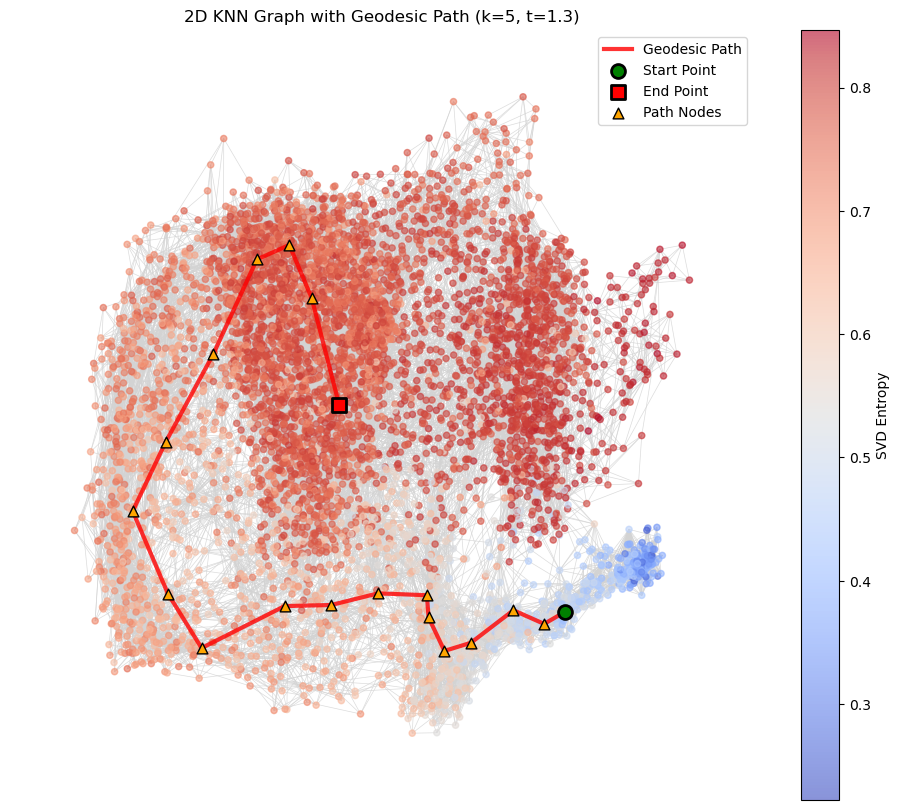
\includegraphics[width=0.8\textwidth]{/home/oliver/text-learning/geodesic.png}
\caption{Geodesic path visualization showing semantic transitions between documents in the diffusion map embedding.}
\label{fig:geodesic}
\end{figure}

The 2D spring layout \cite{spring-layout} visualization in Figure \ref{fig:geodesic} reveals the intrinsic geometric structure of the document manifold through diffusion map embedding. The color gradient represents SVD entropy values, creating a natural "complexity landscape" where blue regions (low entropy, 0.3-0.4) may correspond to foundational concepts, and red regions (high entropy, 0.7-0.8) specialized topics.

The geodesic path (red line with triangular markers) demonstrates a clear semantic progression from the bottom-right (start point, green circle) to the center-left (end point, red square). This trajectory traverses multiple entropy gradients, suggesting the path naturally follows increasing conceptual complexity. Notably, the path avoids the densest red regions, indicating that the algorithm discovers routes through intermediate complexity levels rather than attempting direct transitions between fundamentally different concept spaces.

\subsubsection{Geodesic Path Progression Analysis}

\begin{table}[htbp]
\caption{Geodesic Path from Start to End Point}
\label{tab:geodesic_path}
\begin{tabular}{|c|p{12cm}|c|}
\toprule
Index & Text (first 125 chars) & SVD Entropy \\
\midrule
0 &  Introducing matrices  Published:  Here, I will introduce the three main ways of thinking about matrices. This high-level de ... & 0.4861 \\
1 & Data for Exercise 7.40  Backtoback   Format  A data frame/tibble with 24 observations on two variables  score  a numeric ve ... & 0.5664 \\
2 &  Autoencoder   Difference between generative and discriminative modelling   Generative modelling  Generative modelling  ... & 0.5233 \\
3 &  Measure the uncertainty in deep learning models using dropout  Seminal blog post of Yarin Gal from Cambridge machine learni ... & 0.6269 \\
4 & In today’s post I would like to give you a quick-and-dirty introduction into a neural network architecture type called Autoen ... & 0.5695 \\
5 & Conv Layers  In turn, each neuron in the second conv layer is connected only to neurons located within a small rectangle in t ... & 0.5963 \\
6 &  Chapter 2: Matrices and Linear Algebra¶  import igl import scipy as sp import numpy as np from meshplot import plot, subplo ... & 0.5848 \\
7 &  A practical introduction to GNNs - Part 1  This is Part 1 of an introductory lecture on graph neural networks that I gave f ... & 0.6182 \\
8 &  Generative Adversarial Network (GAN) in TensorFlow - Part 4   The GAN Class and Data Functions  Now that we’re able to im ... & 0.6188 \\
9 &  Lecture 6: Further Examples of Classifiers¶  This week we're discussing more classifiers and their applications.   Suppor ... & 0.6992 \\
10 &  K-Nearest Neighbor from Scratch in Python  Posted by Kenzo Takahashi on Wed 06 January 2016  We are going to implement K-ne ... & 0.6884 \\
11 &  Multi-layer Perceptron (MLP)¶  New in version 0.3.  In this module is stored everything related to Multi-layer perceptron ( ... & 0.6415 \\
12 &  TensorFlow 101  Word2Vec  Shan-Hung Wu  DataLab Fall 2018  TensorFlow is a powerful open source libraray used for large-s ... & 0.7221 \\
13 &  Libraries  import numpy as np import pandas as pd import matplotlib.pyplot as plt import seaborn as sns  sns.set()  matplo ... & 0.6781 \\
14 &  2.1 Three Popular Data Displays   Learning Objective  1. To learn to interpret the meaning of three graphical represent ... & 0.7286 \\
15 &  Machine learning  For the journal, see Machine Learning (journal).  Machine learning is a subfield of computer science and  ... & 0.7235 \\
16 &  Exploring and Understanding Hyperparameter Tuning  Learners use hyperparameters to achieve better performance on particular ... & 0.7651 \\
17 & In this post I’ll talk through the pieces of the tensorflow API most relevant to building recurrent neural networks. The tens ... & 0.7719 \\
18 &  LSTMs  2 minute read     LSTMs to Model Physiological Time Series  Harini Suresh, Nicholas Locascio, MIT   Neural Net ... & 0.7738 \\
\bottomrule
\end{tabular}
\end{table}


Table \ref{tab:geodesic_path} shows the semantic progression along the discovered 19-step path, exhibiting a clear entropy gradient from 0.4861 (basic matrices) to 0.7738 (LSTM networks).

The path reveals a continuous progression through the conceptual landscape, beginning with basic mathematical foundations and gradually transitioning through core machine learning concepts including autoencoders and neural networks, ultimately reaching sophisticated architectures like LSTM networks.

The smooth entropy progression with minimal backtracking demonstrates that diffusion geodesics successfully identify natural learning sequences, automatically discovering pedagogically meaningful pathways.

\section{Discussion}

\subsection{Methodological Advantages}

Our diffusion-based methodology offers several significant advantages over traditional text mining approaches. By treating the text corpus as a manifold with intrinsic geometry, we enable natural distance computations that reflect semantic relationships. The diffusion process naturally incorporates a time parameter, allowing analysis at multiple scales and the discovery of hierarchical relationships. The use of entropy-based similarity measures and diffusion distances ensures that the intrinsic semantic relationships are preserved throughout the analysis. Optimizations using Numba and efficient data structures enable the processing of medium-scale document collections with reasonable computational resources. The geodesic paths and diffusion map embeddings provide results that are not only effective for analysis but also interpretable in terms of semantic relationships and document complexity.

\subsection{Limitations and Future Work}

While our methodology demonstrates promising results, several limitations warrant consideration. The current implementation is suitable for medium-scale corpora, but scaling to very large document collections would require distributed computing approaches or approximate methods for eigendecomposition and distance computations. The method involves several parameters (SVD components, diffusion time, kernel bandwidth) that may require tuning for different domains and corpus characteristics. Additionally, the approach has been validated primarily on mathematical and machine learning content, and evaluation on other domains would strengthen the generalizability claims.

Future work could explore adaptive parameter selection, distributed implementations for large-scale corpora, and validation across diverse text domains to establish broader applicability.

\section{Conclusion}

This work presents a novel framework for text mining that leverages diffusion geometry and information theory to reveal the underlying semantic structure of document corpora. Our approach successfully combines TF-IDF vectorization, SVD-based dimensionality reduction, entropy-based similarity measures, and diffusion processes to create a comprehensive analysis pipeline.

The key innovations include the development of SVD entropy as a measure of document generality and complexity, the use of asymmetric cross-entropy kernels to capture directional semantic relationships, and the computation of semantic geodesics that represent meaningful learning pathways between concepts.

Evaluation on a mathematical machine learning corpus demonstrates the method's effectiveness in discovering semantic relationships, characterizing document complexity, and finding interpretable paths between conceptually distant topics. The approach provides both quantitative measures through diffusion distances and qualitative insights through geodesic path analysis.

The framework opens new possibilities for educational technology, where semantic geodesics could guide personalized learning paths, and for knowledge discovery, where the geometric structure of document collections can reveal hidden relationships and progression patterns in specialized domains.

\begin{thebibliography}{9}

\bibitem{coifman2006diffusion}
Coifman, R. R., \& Lafon, S. (2006). Diffusion maps. \textit{Applied and computational harmonic analysis}, 21(1), 5-30.

\bibitem{salton1988term}
Salton, Gerard, and Christopher Buckley. "Term-weighting approaches in automatic text retrieval." Information processing \& management 24.5 (1988): 513-523.

\bibitem{deerwester1990indexing}
Deerwester, S., Dumais, S. T., Furnas, G. W., Landauer, T. K., \& Harshman, R. (1990). Indexing by latent semantic analysis. \textit{Journal of the American society for information science}, 41(6), 391-407.

\bibitem{boutsidis2008svd}
Boutsidis, C., \& Gallopoulos, E. (2008). SVD based initialization: A head start for nonnegative matrix factorization. \textit{Pattern recognition}, 41(4), 1350-1362.

\bibitem{grosset2021openwebmath}
Paster, Keiran, et al. "Openwebmath: An open dataset of high-quality mathematical web text." arXiv preprint arXiv:2310.06786 (2023).

\bibitem{grootendorst2022bertopic}
Grootendorst, Maarten. "BERTopic: Neural topic modeling with a class-based TF-IDF procedure." arXiv preprint arXiv:2203.05794 (2022).

\bibitem{djikstra}
Dijkstra, Edsger W. "A note on two problems in connexion with graphs." Edsger Wybe Dijkstra: his life, work, and legacy. 2022. 287-290.

\bibitem{spring-layout}
Kobourov, Stephen G. "Spring embedders and force directed graph drawing algorithms." arXiv preprint arXiv:1201.3011 (2012).

\end{thebibliography}

\end{document}